\documentclass{beamer}
\usetheme{metropolis}           % Use metropolis theme
\newcommand{\thchdir}{../code/3chains}
\newcommand{\twchdir}{../code/2chains}

\title{Comparative analysis of water structure
for HIV-1 Reverse transcriptase in
complex with DMP-266 (Efavirenz)}
\date{July 6, 2022}
\author{Filippo Conforto}
\institute{Università degli studi di Padova \\ Molecular Simulations}
\begin{document}
\maketitle

\section{Introduction}
\begin{frame}
    The molecular complex \textbf{1fk9} represents an application of \textbf{Efavirenz} (EFZ) as inhibitor of reverse transcriptase. Its structure consists of:
    \begin{itemize}
        \item \textbf{Chain A}  (588-1130 of Uniprot P04585, wild type).
        \item \textbf{Chain B}  (588 to 1027 of Uniprot P04585)
        \item \textbf{EFZ}
    \end{itemize}
\end{frame}
\begin{frame}
    \begin{figure}
        \centering
        \includegraphics[width=0.5\textwidth]{../figures/water.png}
        \caption{Protein complex, water molecules are represented by the blue beads according to the VdW radius, EFZ is represented in red, Chain A in green, and Chain B in gold. \label{fig:total}}
    \end{figure}
\end{frame}

\section{Methods}
\begin{frame}{Structural analysis}
    In order to simulate the complex the two unknown residues for amber were \textbf{modelled}  following these steps:

    \begin{itemize}
        \item Hydrogen addition
        \item Charges computation
        \item General force field (gaff) assignment
    \end{itemize}

    To ease computations also, were created two configurations: \textbf{Chain A + EFZ}, \textbf{Chain B + EFZ}
\end{frame}

\begin{frame}{Active residues}
    To get a reference for the analysis of the substrate in the studied solution, \textbf{active residues}  were located by checking for atom distant at most \textbf{4 \AA}  from the EFZ's atoms.

    In this way it was possible to cover any possible type of bond between the substrate and the possible active residues.
\end{frame}

\begin{frame}
    \begin{figure}
        \centering
        \includegraphics[width=\textwidth]{../figures/act_res.png}
        \caption{Labelled active residues found in the proximity of EFZ (brown beads).  \label{fig:actres}}
    \end{figure}
\end{frame}

\begin{frame}{Model preparation, solvent and minimization}
    After having individuated the active residues it was possible to load the model using the predefined force field library ("\textbf{ff99SB}") along with the user defined libraries for \textbf{CSD}  and \textbf{EFZ}.

    This solute was then inserted in a pre-equilibrated water solution, using \textbf{TIP3P} library and then minimized to the configuration with minimum energy.
\end{frame}

\begin{frame}
    \begin{figure}
        \centering
        \includegraphics[width=0.8\linewidth, clip, trim= 0 0 0 0]{../figures/chain_a_efz_solv.png}
        \caption{Chain A + EFZ configuration in solution after minimization. In red can be seen the EFZ residue, while the purple beads represent the Na+ ions. \label{fig:chain_a_efz_solv}}
    \end{figure}
\end{frame}

\begin{frame}
    \begin{figure}
        \centering
        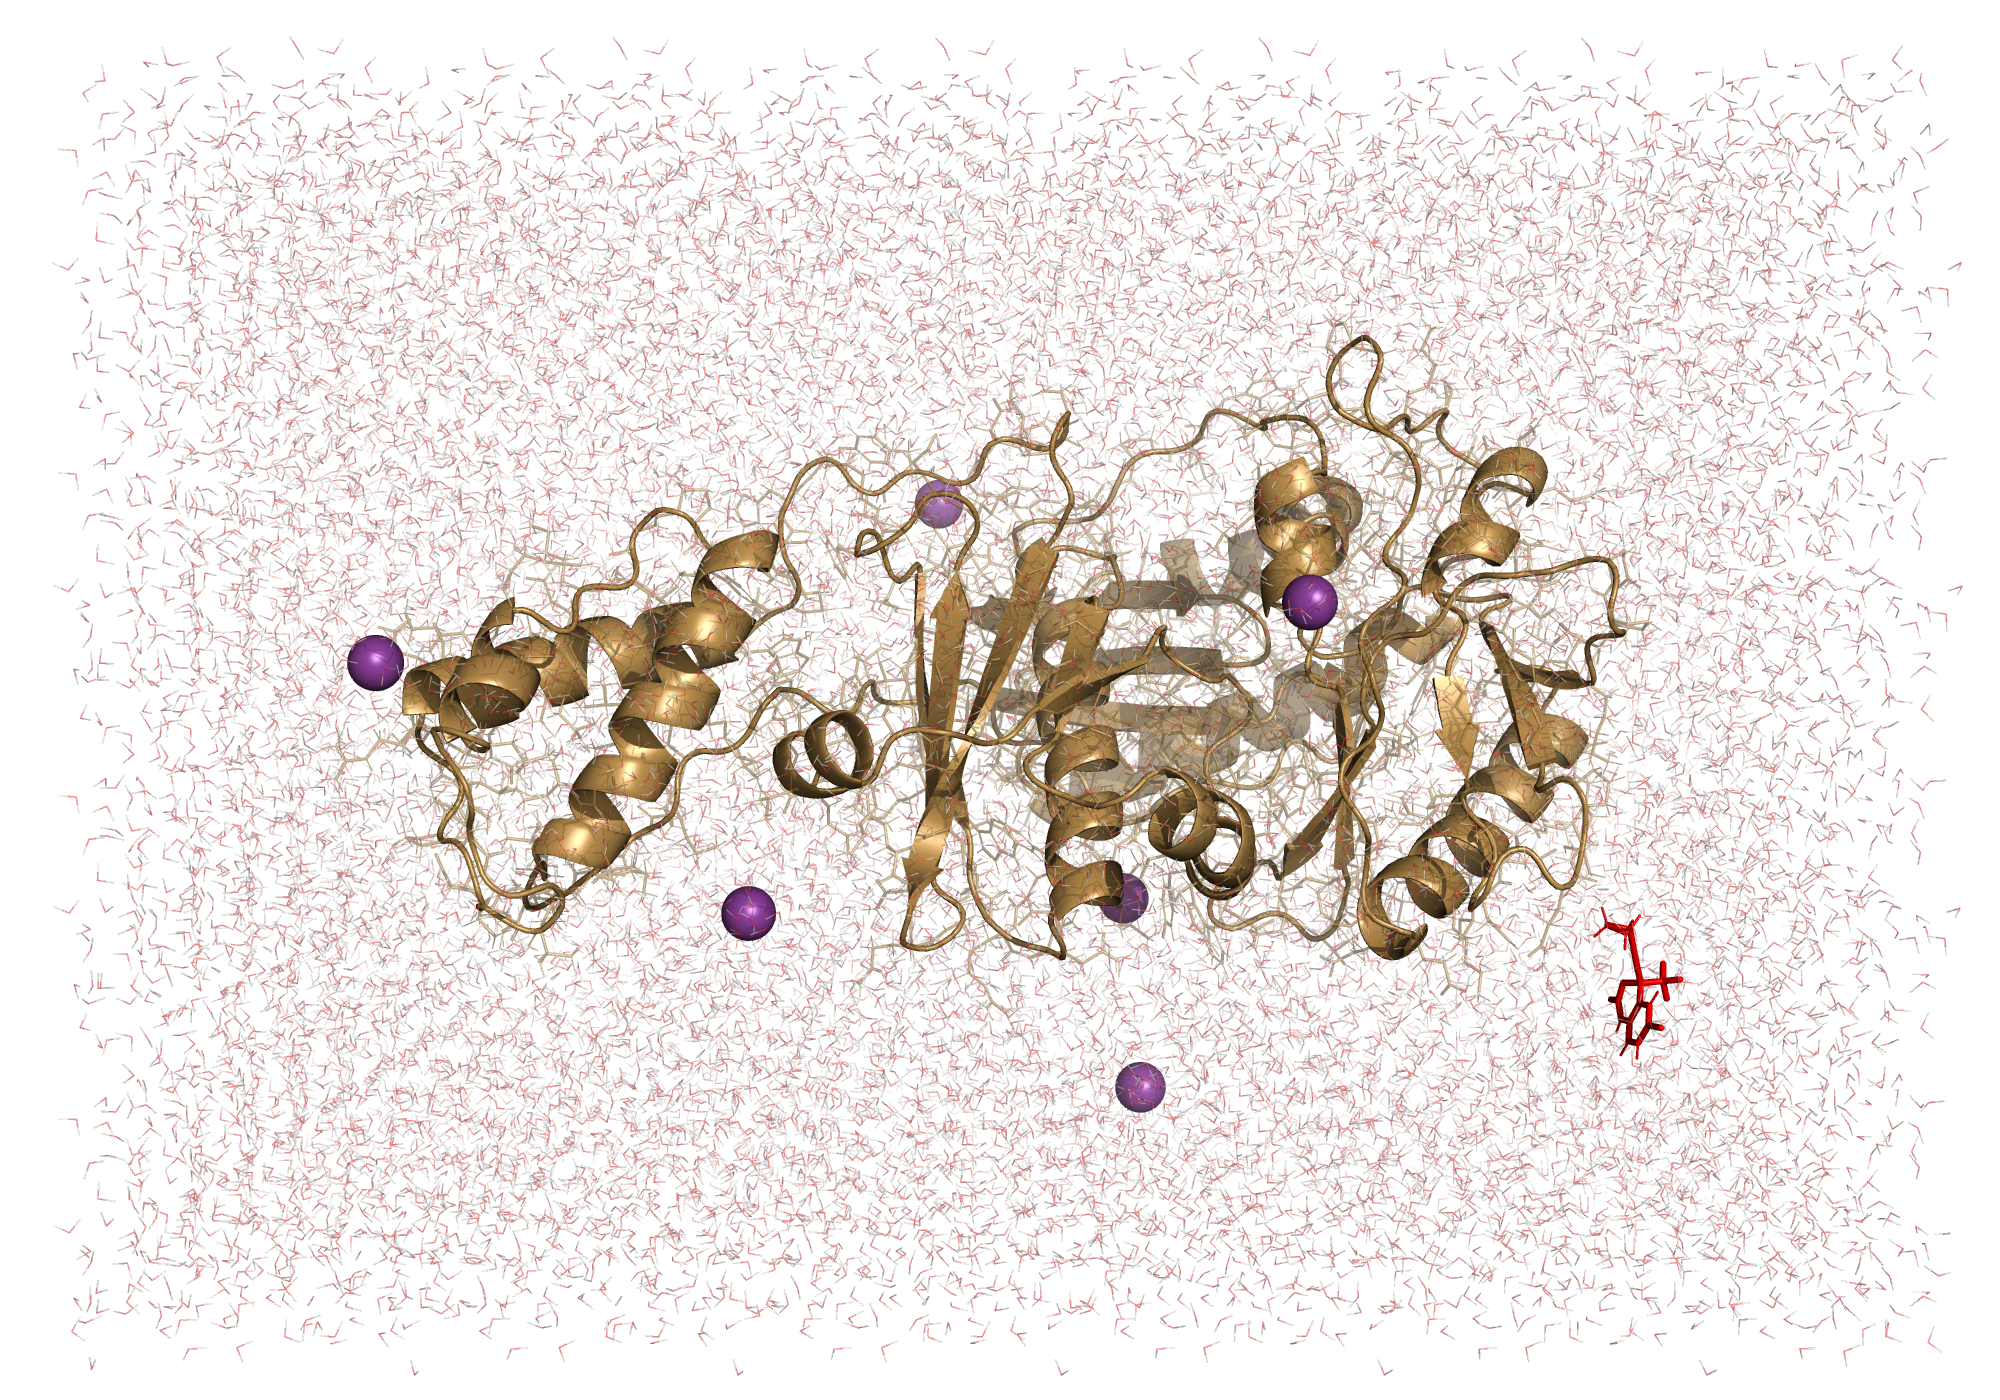
\includegraphics[width=0.8\linewidth, clip, trim= 0 0 0 0]{../figures/chain_b_efz_solv.png}
        \caption{Chain B + EFZ configuration in solution after minimization. In red can be seen the EFZ residue, while the purple beads represent the Cl- ions.\label{fig:chain_b_efz_solv}}
    \end{figure}
\end{frame}

\begin{frame}{Heating and simulation}
    Starting from the minimized configuration it was possible to \textbf{heat} the system up to 298 K and then simulate the behavior at \textbf{fixed temperature}.

    Both the simulations were run using \textbf{periodic boundary conditions} and a cutoff at 15 \AA. The timesteps instead were different and fixed respectively at 2 and 1 fs, with a total simulation time of 20 ps and 100 ps.
\end{frame}

\section{Results}
\begin{frame}{Radial distribution function and coordination number}
    These two quantities were calculated to study the distribution of water around the active residues and the substrate. The formulas used were:
    \begin{equation}
        g(r) = \frac{V}{4\pi r^2 \Delta r N^2}\sum_i n_i(r,\Delta r)
        \label{eq:gofr}
    \end{equation}
    \begin{equation}
        K(r) = 4\pi \rho \int_{0}^{r_c} dr \, r^2 g(r)
        \label{eq:kofr}
    \end{equation}
\end{frame}

\begin{frame}{Chain B + EFZ}
    \begin{figure}[H]
        \centering
        \includegraphics[width=\textwidth]{../figures/b_chain_act.pdf}
        \caption{Radial distribution function g(r) and running coordination number K(r) of water around active sites for the configuration Chain B + EFZ. g(r) in dark blue, K(r) in light blue.\label{fig:gofr_chain_b_efz}}
    \end{figure}
\end{frame}

\begin{frame}{Chain A + EFZ - Shells}
    \begin{figure}
        \centering
        \includegraphics[width=0.49\textwidth, clip, trim= 300 550 600 0]{../figures/a_chain_act.pdf}
        \includegraphics[width=0.49\textwidth, clip, trim= 600 550 300 0]{../figures/a_chain_act.pdf}
        \caption{Radial distribution function g(r) and running coordination number K(r) of water around active sites for the configuration Chain A + EFZ. g(r) in dark blue, K(r) in light blue.\label{fig:gofr_chain_a_efz_1}}
    \end{figure}
\end{frame}

\begin{frame}{Chain A + EFZ - Hydrophobicity}
    \begin{figure}
        \centering
        \includegraphics[width=0.49\textwidth, clip, trim= 0 185 900 365]{../figures/a_chain_act.pdf}
        \includegraphics[width=0.49\textwidth, clip, trim= 900 0 0 550]{../figures/a_chain_act.pdf}
        \caption{Radial distribution function g(r) and running coordination number K(r) of water around active sites for the configuration Chain A + EFZ. g(r) in dark blue, K(r) in light blue.\label{fig:gofr_chain_a_efz_2}}
    \end{figure}
\end{frame}
\begin{frame}{RSMD}
    \begin{figure}[H]
        \centering
        \includegraphics[width=\textwidth]{../figures/rmsd.pdf}
        \caption{Global RSMD for the Chain A + EFZ case (a) and the Chain B + EFZ case (b).\label{fig:rmsd}}
    \end{figure}
\end{frame}


\begin{frame}{RSMF}
    \begin{figure}[H]
        \centering
        \includegraphics[width=\textwidth]{../figures/rmsf_efz.pdf}
        \caption{RSMF of the EFZ residue for the Chain A + EFZ case (a) and the Chain B + EFZ case (b).\label{fig:rmsf}}
    \end{figure}
\end{frame}

\begin{frame}
    \begin{figure}
        \centering
        \includegraphics[width=0.4\textwidth]{../figures/efz.png}
        \caption{EFZ ligand.\label{fig:efz}}
    \end{figure}

    The atoms with largest RMSF correspond to the \textbf{carbons}  in the triangular formation, along with the \textbf{chlorine}  in the aromatic ring. 
\end{frame}

\begin{frame}{Distance from active site}
    \begin{figure}[H]
        \centering
        \includegraphics[width=\textwidth]{../figures/dis_chain_act.pdf}
        \caption{EFZ distance from the active site for the Chain A + EFZ case (a) and the Chain B + EFZ case (b).\label{fig:dist}}
    \end{figure}
\end{frame}

\section{Conclusions}

\begin{frame}

    \begin{itemize}
        \item The values of \textbf{g(r)}  and \textbf{K(r)} allowed detecting \textbf{hydrophobicity}  phenomenons along with the presence of \textbf{hydration cells}  around some residues.
        \item The calculation of RSMD instead showed some stability on the global structure distance from the original configuration, while RSMF and distance computations on EFZ allowed understanding more of the atomic and global movement of EFZ, showing the presence of different \textbf{configurations} and atoms with large \textbf{movement freedom}.
        \item Finally, the distance of EFZ from the active sites allowed appreciating stable configuration and transient ones in both the simulated complexes.
    \end{itemize}

\end{frame}

\begin{frame}{}
    \centering \Large
\emph{Thank you!}
  \end{frame}
  
\end{document}




